\subsection*{Running only MPI or openMP}
\begin{figure}[h!]
			\centering
			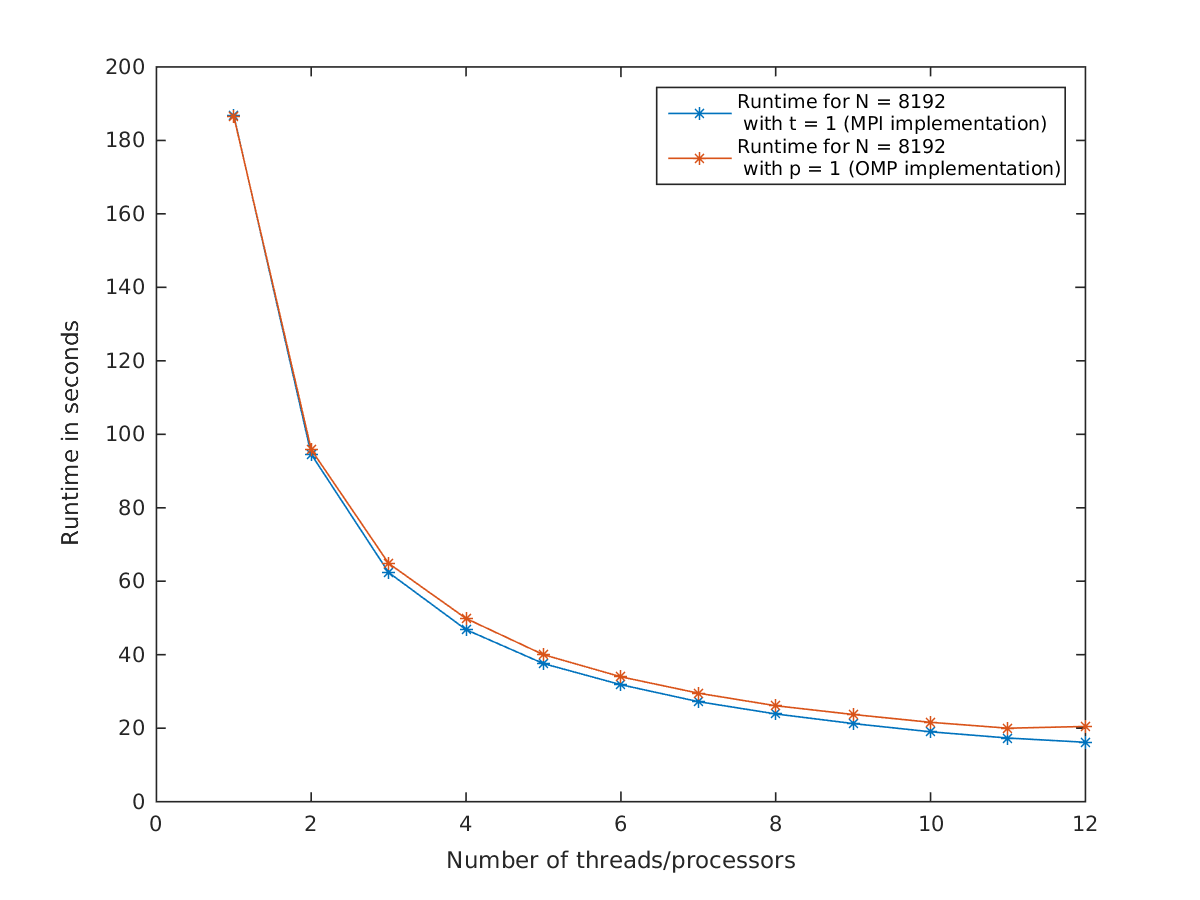
\includegraphics[width=0.7\textwidth]{./figures/runtime_either_MPI_OMP}
			\caption{Runtime for MPI and OMP program.}
			\label{fig:MPIvsOMP}
\end{figure}
We first run our code both as a pure MPI and as a pure OpenMP program on one node to look at runtime. From figure \ref{fig:MPIvsOMP} we see that the runtime is equal for $t = p = 1$, as it obviously should be since this is the serial implementation. Then, the runtime decreases as $p$ and $t$ increases, as it should. In other words, we get a good speedup for both parallelization methods given that we are at one node. 


\subsection*{Optimal number of nodes with MPI}

The next question then becomes: given a number of processors, which number of nodes will work best? The results are presented in figure \ref{fig:bestnodes}.
\begin{figure}[h]
\centering
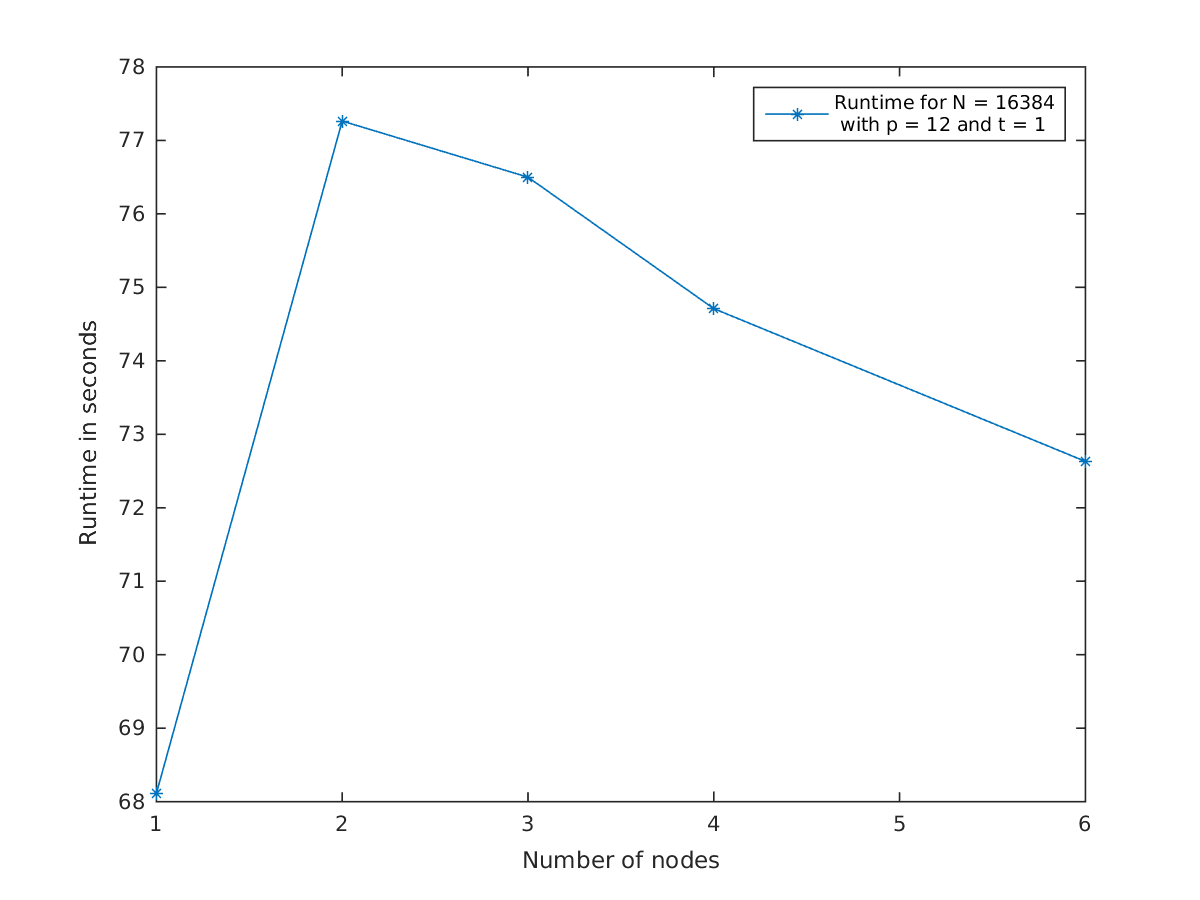
\includegraphics[width=0.7\textwidth]{./figures/bestnodes}
\caption{Running the problem on a different amount of nodes with the combined number of processors to be 12.}
\label{fig:bestnodes}
\end{figure}
The clearly best result is if we keep all the processing on a single node, but the moment we spread out to two or more nodes we get a speedup for every new node we add (at least till six nodes). We attribute this to be the limiting factor of bandwidth between the nodes. We will get much more efficient use of the bandwidth if we spread our data across multiple nodes. The implementation only transfers data in the transpose function, but then again it transfers a lot of data at the same time. It's therefore natural that we reach the bandwidth cap.


\subsection*{Hybrid vs pure distributed memory model}
To test the hybrid and the pure distributed memory model we do a few runs on Kongull with the following settings such that $n = 16384$,  $t\cdot p = 36$ and $p = \{1, 2, 3, 4, 6, 9, 12, 18, 36\}$. We allocate six nodes so we at least get some of the performance improvement from spreading the processing out to more nodes.
\begin{figure}[h]
\centering
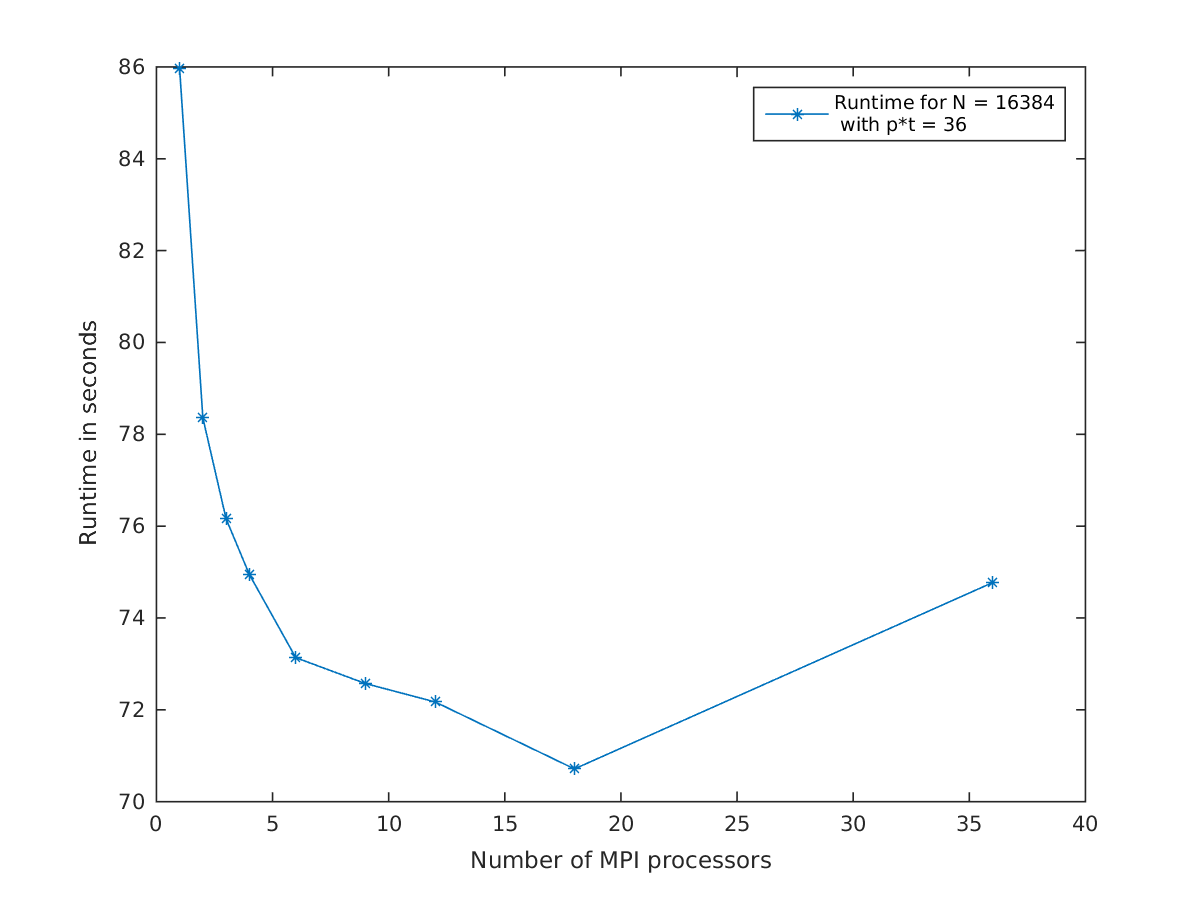
\includegraphics[width=0.7\textwidth]{./figures/pt36}
\caption{Runtime with different numbers for MPI processors and openMP threads with $p\cdot t = 36$.}
\label{fig:runtime}
\end{figure}
As seen in figure \ref{fig:runtime} the pure distributed model outclasses the hybrid model. This may be the case since the problem is pretty local in the sense that we don't need many MPI calls. We need, however, quite a few openMP calls. It seems reasonable that for this problem the pure distributed memory model works best since we only need to send data between nodes twice, and it may be most efficient to just spread the data all the way from the beginning. Figure \ref{fig:MPIvsOMP} shows that even when using just one node (and twelve cores) the pure distributed model performs marginally better than the hybrid model.


\subsection*{Speedup and parallel efficiency}
The speedup, $S_P$ is is defined as the ratio between the solution time on one single processor divided by the solution time on $P$ processors, $S_p=\frac{T_1}{T_P}$. Ideally $S_P$ should be $S_P=T_1P$. When we study figure \ref{fig:speedup}, that is the plot of the speedup of our code, we see that in the beginning this happens, but with more that with more processors the speedup still increases, but not as much.
\\ \\
The speedup increases because the all computational tasks are spread to all the processors so the computing task for each processor is reduced. When the problem increases and the number of processors increases the communication between the processors increases. At one point the time used to communicate increases so much that it reduces the run time the speedup. We have not yet encountered this, but we assume it'll come soon if we continue to increase the problem size.

\begin{figure}[h]
        \centering
        \begin{subfigure}[b]{0.45\textwidth}
			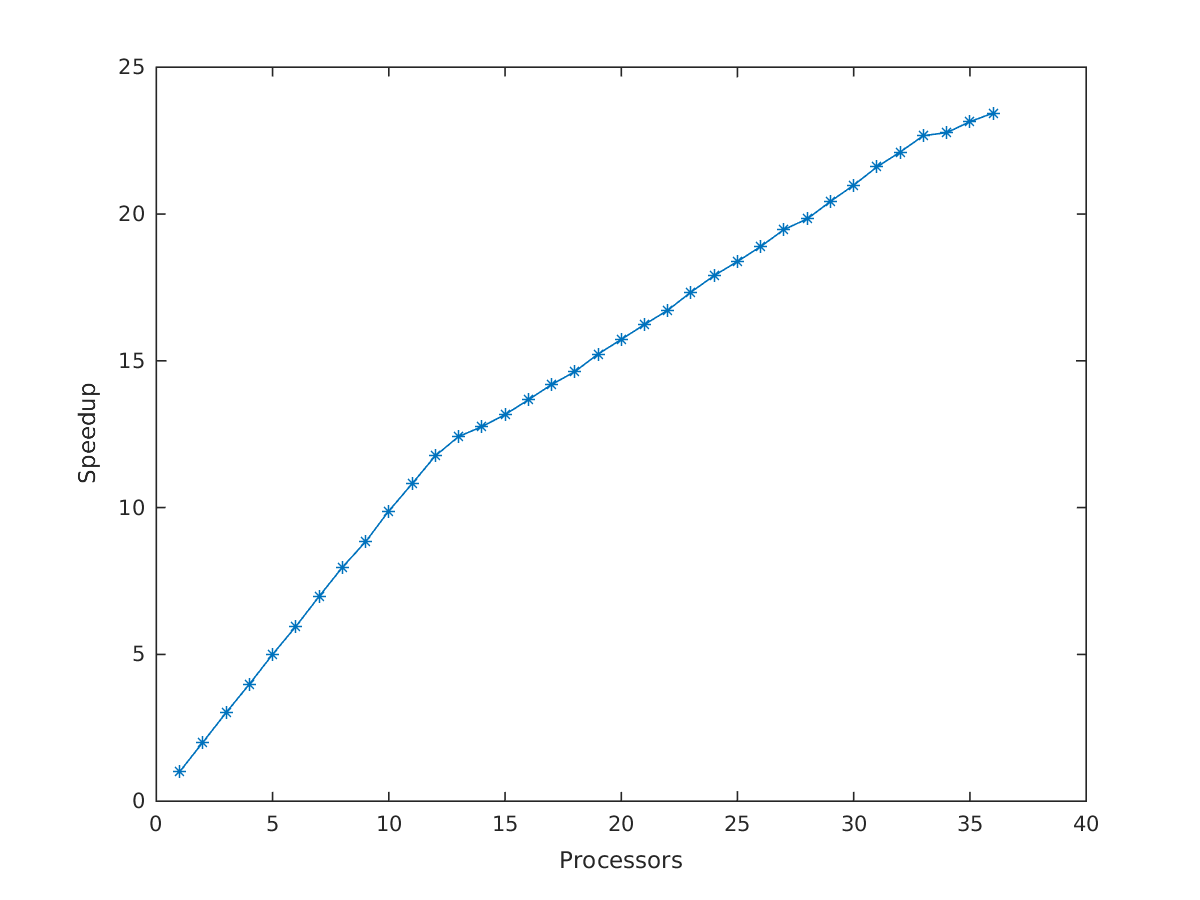
\includegraphics[width=\textwidth]{./figures/speedup}
			\caption{Parallel speedup.}
			\label{fig:speedup}
        \end{subfigure}
        ~ %add desired spacing between images, e. g. ~, \quad, \qquad, \hfill etc.
          %(or a blank line to force the subfigure onto a new line)
        \begin{subfigure}[b]{0.45\textwidth}
			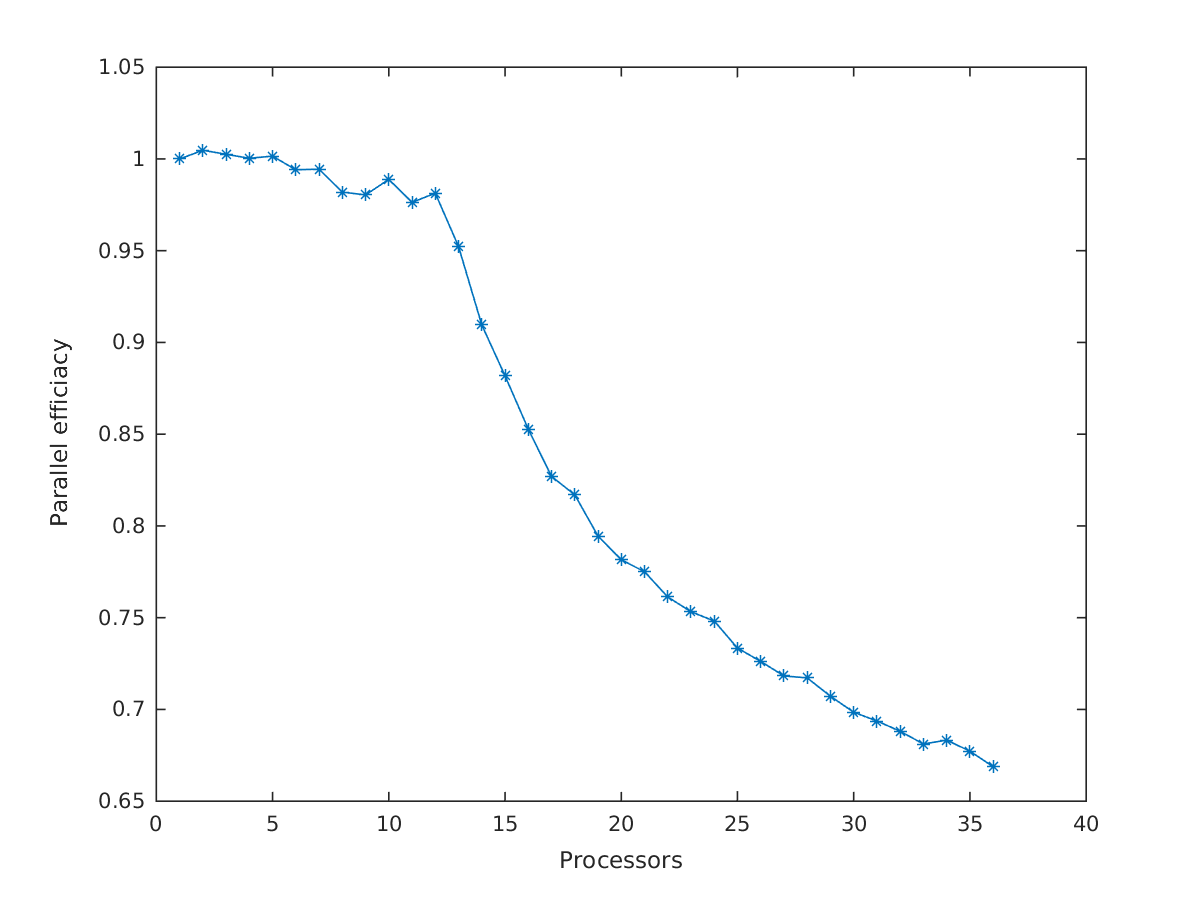
\includegraphics[width=\textwidth]{./figures/efficiacy}
			\caption{Parallel efficiency.}
			\label{fig:efficiacy}
        \end{subfigure}%
        \caption{Parallel speedup and efficiency for the pure distributed memory model. We assigned 6 nodes to tackle this problem.}
        \label{fig:analysis}
\end{figure}

As can be seen in figure \ref{fig:efficiacy} the parallel efficiency, defined as $\eta_P=\frac{S_P}{p}$, is almost ideal as long we only use a single node with 12 processors. With more than 12 processors the efficiency drops, but the speedup still makes it worth it. We assume this happens because the network overhead of using more than one node inhibits the efficiency more than the overhead of transporting things inside the node itself. According to the linear model of data transfer latency we would say that the latency (the constant) is larger when communicating between nodes than when we communicate in-node.


\subsection*{How does runtime scale with N}
\begin{figure}[h!]
			\centering
			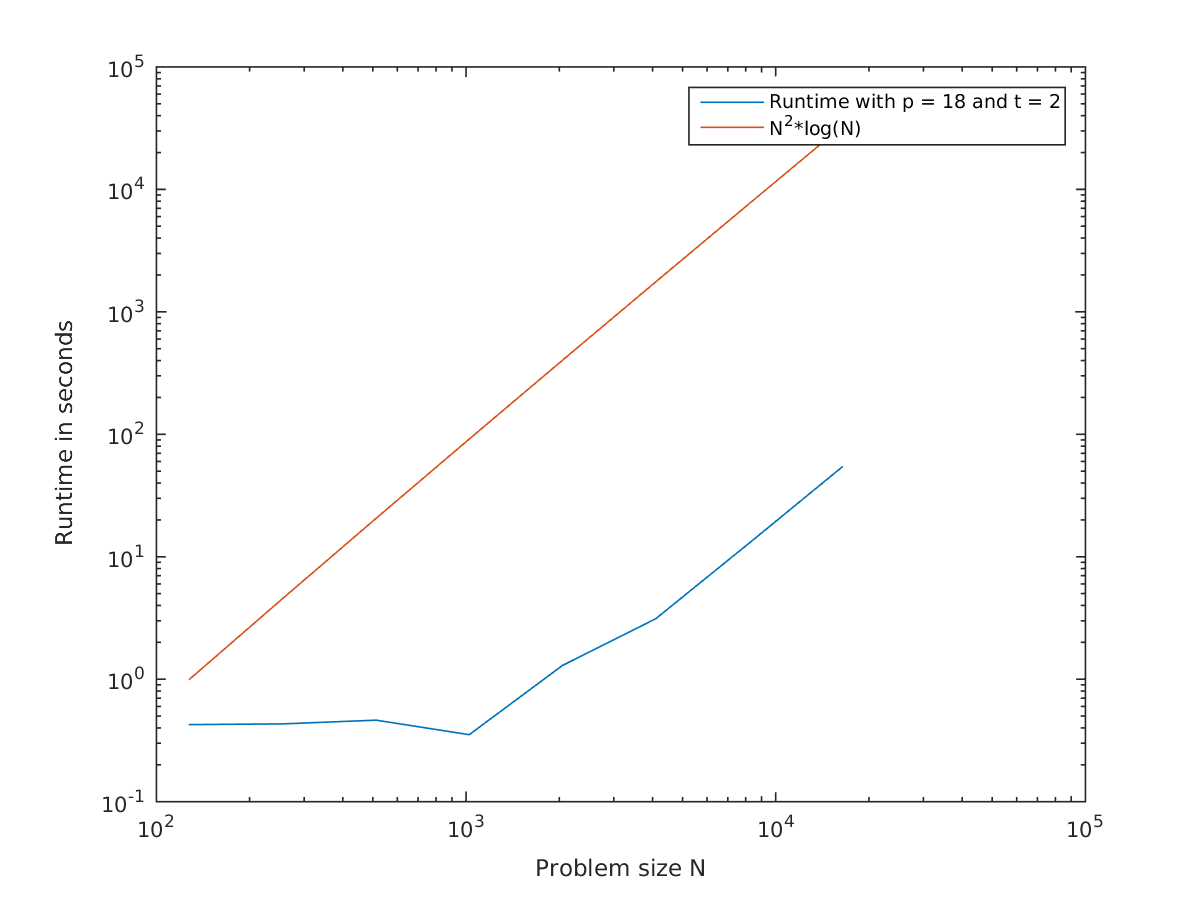
\includegraphics[width=0.7\textwidth]{./figures/runtimeN}
			\caption{Runtime with increasing problem size.}
			\label{fig:runtimeN}
\end{figure}
Next, we study how the runtime of our program scales with the problem size $N$. From the theory, we know that the runtime should be of order $\mathcal{O}(N^2\log(N))$. We observe from figure \ref{fig:runtimeN} that the runtime appear to go towards the expected order as $N$ increases.
